\documentclass{article}
\usepackage{import}
\import{../../lib/latex/}{wgmlgz}


\begin{document}

\itmo[
  variant=129,
  labn=7,
  discipline=Основы профессиональной деятельности,
  group=P3115,
  student=Владимир Мацюк,
  teacher=Абузов Ярослав Александрович,
  logo=../../lib/img/itmo.png
]


\section{Текст задания}

Синтезировать цикл исполнения для выданных преподавателем команд. Разработать тестовые программы, которые проверяют каждую из синтезированных команд. Загрузить в микропрограммную память БЭВМ циклы исполнения синтезированных команд, загрузить в основную память БЭВМ тестовые программы. Проверить и отладить разработанные тестовые программы и микропрограммы.



\begin{enumerate}
  \item SHR X - сдвиг аккумулятора вправо на X разрядов, 15 разряд заполняется значением 0, количество сдвигов содержится в коде команды. Признаки N/Z/V/C не устанавливать
  \item Код операции - 0F8X (000011111000xxxx)
  \item Тестовая программа должна начинаться с адреса $0221_{16}$
\end{enumerate}

\section{Исходный код синтезируемой команды}

\begin{center}
  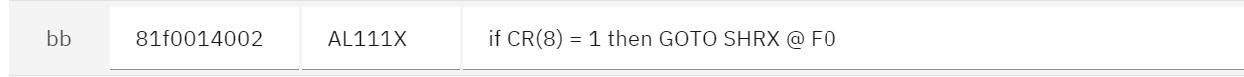
\includegraphics{1.png}
  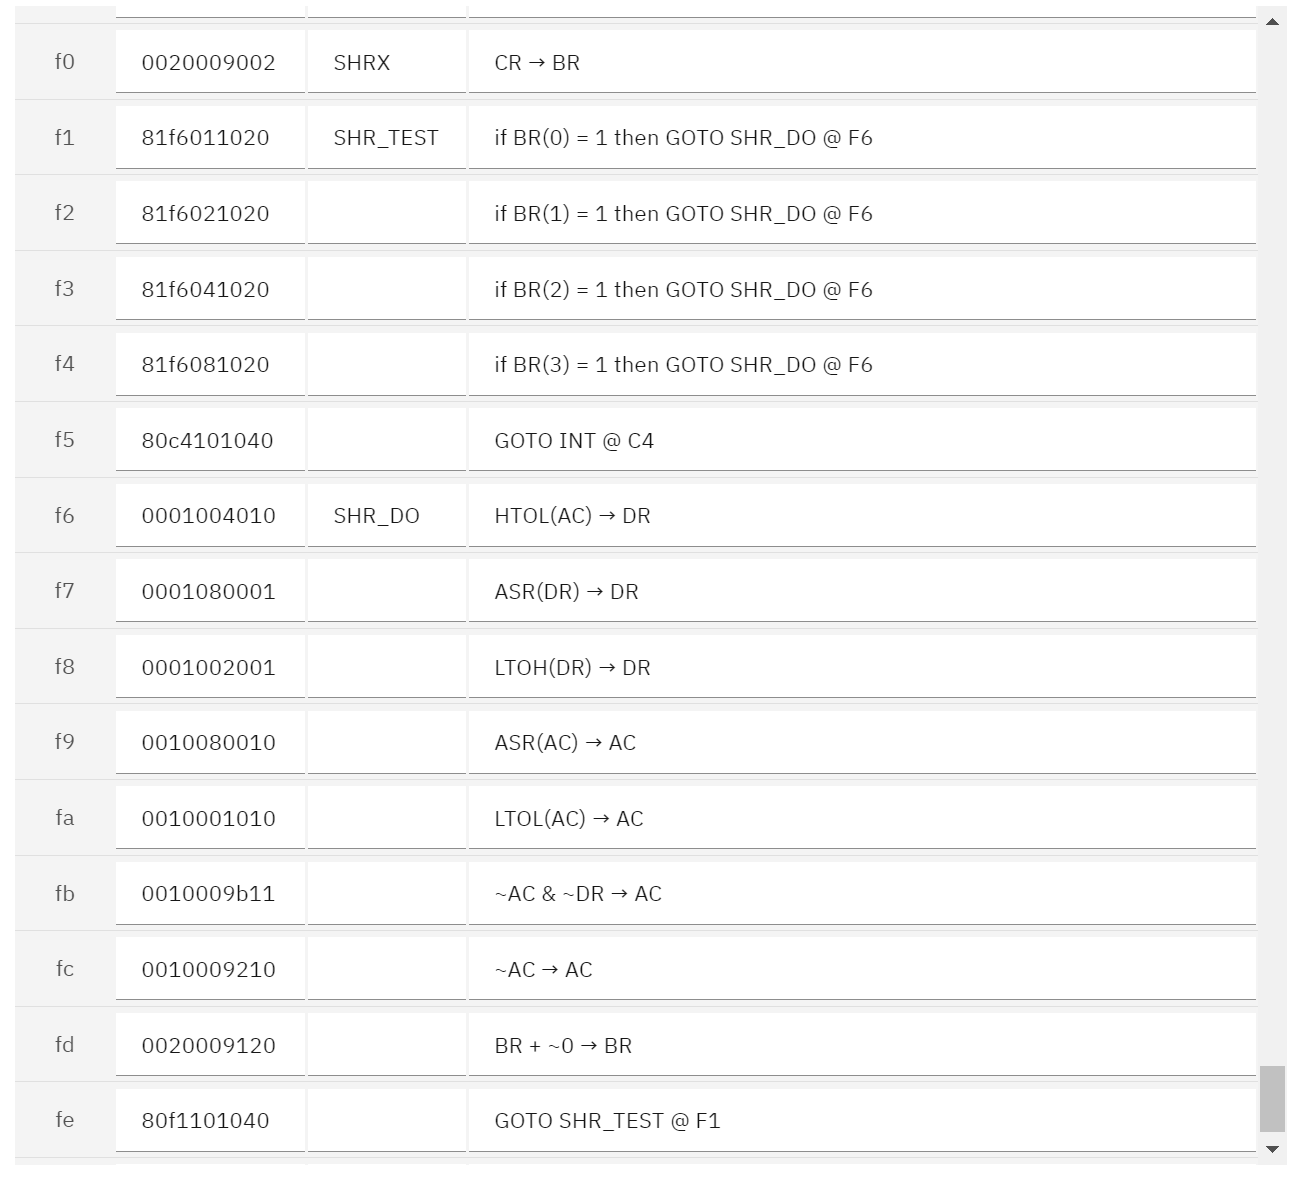
\includegraphics{2.png}
\end{center}


\section{Программа}

\lstinputlisting{code.bcomp}

\section{Описание программы}
Программа тестируем синтезированную команду на трех разных тестах и записывает 1, если результат сходится и 0, если нет.




\section{Методика проверки (Подготовка к проверке)}
\begin{enumerate}

  \item Скачать код с Github: https://github.com/Wgmlgz/itmo/tree/main/opd/l7
  \item Открыть БЭВМ в формате cli или dual “java –Dmode=cli –jar bcomp-ng-ex.jar”
  \item Открыть help “?”
  \item На основе help и таблицы микрокоманд перенести нужные микрокоманды в БЭВМ
  \item Открыть режим ввода Assembler “asm”
  \item Загрузить команды Assembler в БЭВМ
  \item Написать после кода Assembler END и нажать Enter
\end{enumerate}

\section{Методика проверки синтезированной программы:}
\begin{enumerate}
  \item Ввести комманды ru, s
  \item Дождаться остановы.
  \item Удостовериться, что значения правильные
\end{enumerate}

\section{Сопоставление полученного и теоретического результата}

\begin{center}
  \begin{tabular}{|c|c|c|c|c|c|}\hline
    Ячейка с результатом & Число & Сдвиг & Теоретический результат & Полученный результат \nl
    RES1                 & 0000  & 1     & 0000                    & 0000  \nl
    RES2                 & 0030  & 4     & 0003                    & 0003 \nl
    RES3                 & F000  & 8     & 00F0                    & 00F0 \nl
  \end{tabular}
\end{center}

\section{Вывод}

В ходе выполнения лабораторной работы я изучил алгоритм синтеза собственной команды БЭВМ с помощью микропрограмм и методику проверки сделанной программы

\end{document}
